\documentclass[aspectratio=169,12pt]{beamer}
\usepackage{amsmath}
\usepackage{amssymb}
\usepackage[most]{tcolorbox}
\usepackage{tikz}
\usepackage{graphicx}
\usepackage[sfdefault,lf]{FiraSans}
\renewcommand{\familydefault}{\sfdefault}
\setlength{\parindent}{0pt}
\everymath{\displaystyle}

\setbeamertemplate{navigation symbols}{}
\setbeamertemplate{footline}{}
\setbeamertemplate{headline}{}

\definecolor{mmpageWhite}{HTML}{FCFBF7}
\definecolor{mmtanSoft}{HTML}{F7F5EF}
\definecolor{mmgreenDeep}{HTML}{244B2C}
\definecolor{mmgreenLeaf}{HTML}{5D8A56}
\definecolor{mmgreenSoft}{HTML}{E4EFD9}
\definecolor{mmtext}{HTML}{163221}

\setbeamercolor{background canvas}{bg=mmpageWhite}
\setbeamercolor{normal text}{fg=mmtext,bg=mmpageWhite}

\newtcolorbox{MMProblemCard}[1][]{enhanced,breakable=false,colback=white,colframe=black,boxrule=1.5pt,arc=8pt,left=5pt,right=5pt,top=4pt,bottom=4pt,before skip=0pt,after skip=0pt,height=0.245\textheight,valign=top,#1}
\newcommand{\KoruIcon}{\raisebox{-0.2em}{
\includegraphics[height=1.05em]{../../SITE/header-logo.png}}}
\newcommand{\HoeIcon}{\raisebox{-0.2em}{
\includegraphics[height=1.05em]{../../SITE/hoe.png}}}
\newcommand{\ScaffoldIcons}[1]{\ifcase#1\or \HoeIcon\or \HoeIcon\hspace{0.22em}\KoruIcon\or \KoruIcon\hspace{0.22em}\KoruIcon\hspace{0.22em}\KoruIcon\fi}
\newcommand{\WorksheetTitle}[2]{%
  {\colorbox{mmtanSoft}{\parbox[c][2.0em][c]{0.975\linewidth}{%
    \hspace{0.25em}{\Large\bfseries\textcolor{mmgreenDeep}{#1}\hfill\ScaffoldIcons{#2}}}}
  \par\vspace{0.08em}{\color{mmgreenLeaf}\rule{\linewidth}{2.0pt}}\par\vspace{0.04em}}
}
\newcommand{\MMProblem}[2]{\begin{MMProblemCard}\raggedright\small\textbf{#1.} #2\par\end{MMProblemCard}}

\setbeamertemplate{background}{
 \begin{tikzpicture}[remember picture,overlay]
 \draw[black,line width=1.5pt,rounded corners=10pt]
 ([xshift=0.45cm,yshift=-0.45cm]current page.north west)
 rectangle
 ([xshift=-0.45cm,yshift=0.45cm]current page.south east);
 \end{tikzpicture}
}

% Default worksheet generation rules:
% use notes-style beamer pages
% use bordered cards for individual problems
% target 9 problems per frame in a 3x3 grid
% target 3 frames per scaffold by default where content allows

\begin{document}\begin{frame}[t]
\WorksheetTitle{Build Tasks}
\vspace{-0.18em}
\begin{columns}[T,onlytextwidth]
\begin{column}{0.32\textwidth}\MMProblem{1}{Find \mbox{$x$}.\\[0.4em]
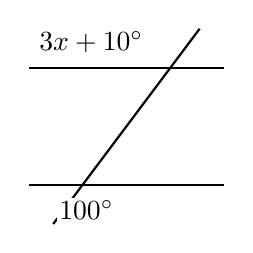
\begin{tikzpicture}[scale=0.62,baseline=(current bounding box.center)]
\draw[thick] (-2,1.2)--(2,1.2);
\draw[thick] (-2,-1.2)--(2,-1.2);
\draw[thick] (-1.5,-2)--(1.5,2);
\node[fill=white,inner sep=1pt] at (-0.72,1.72) {$3x+10^\circ$};
\node[fill=white,inner sep=1pt] at (-0.82,-1.72) {$100^\circ$};
\end{tikzpicture}}\end{column}
\begin{column}{0.32\textwidth}\MMProblem{2}{Find \mbox{$y$}.\\[0.4em]
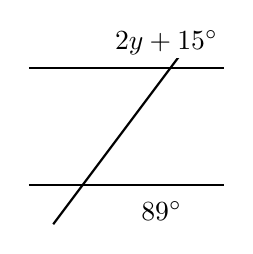
\begin{tikzpicture}[scale=0.62,baseline=(current bounding box.center)]
\draw[thick] (-2,1.2)--(2,1.2);
\draw[thick] (-2,-1.2)--(2,-1.2);
\draw[thick] (-1.5,-2)--(1.5,2);
\node[fill=white,inner sep=1pt] at (0.82,1.72) {$2y+15^\circ$};
\node[fill=white,inner sep=1pt] at (0.72,-1.72) {$89^\circ$};
\end{tikzpicture}}\end{column}
\begin{column}{0.32\textwidth}\MMProblem{3}{Find \mbox{$a$}.\\[0.4em]
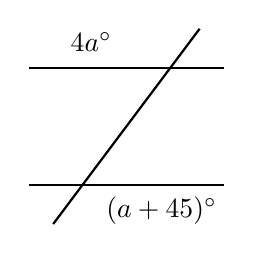
\begin{tikzpicture}[scale=0.62,baseline=(current bounding box.center)]
\draw[thick] (-2,1.2)--(2,1.2);
\draw[thick] (-2,-1.2)--(2,-1.2);
\draw[thick] (-1.5,-2)--(1.5,2);
\node[fill=white,inner sep=1pt] at (-0.72,1.72) {$4a^\circ$};
\node[fill=white,inner sep=1pt] at (0.72,-1.72) {$(a+45)^\circ$};
\end{tikzpicture}}\end{column}
\end{columns}
\vspace{0.45em}
\begin{columns}[T,onlytextwidth]
\begin{column}{0.32\textwidth}\MMProblem{4}{Find \mbox{$b$}.\\[0.4em]
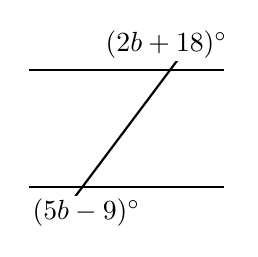
\begin{tikzpicture}[scale=0.62,baseline=(current bounding box.center)]
\draw[thick] (-2,1.2)--(2,1.2);
\draw[thick] (-2,-1.2)--(2,-1.2);
\draw[thick] (-1.5,-2)--(1.5,2);
\node[fill=white,inner sep=1pt] at (0.82,1.72) {$(2b+18)^\circ$};
\node[fill=white,inner sep=1pt] at (-0.82,-1.72) {$(5b-9)^\circ$};
\end{tikzpicture}}\end{column}
\begin{column}{0.32\textwidth}\MMProblem{5}{Find \mbox{$m$}. The marked pair are co-interior.\\[0.4em]
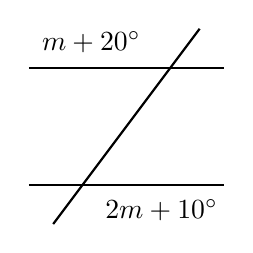
\begin{tikzpicture}[scale=0.62,baseline=(current bounding box.center)]
\draw[thick] (-2,1.2)--(2,1.2);
\draw[thick] (-2,-1.2)--(2,-1.2);
\draw[thick] (-1.5,-2)--(1.5,2);
\node[fill=white,inner sep=1pt] at (-0.72,1.72) {$m+20^\circ$};
\node[fill=white,inner sep=1pt] at (0.72,-1.72) {$2m+10^\circ$};
\end{tikzpicture}}\end{column}
\begin{column}{0.32\textwidth}\MMProblem{6}{Find \mbox{$n$}. The marked pair are co-interior.\\[0.4em]
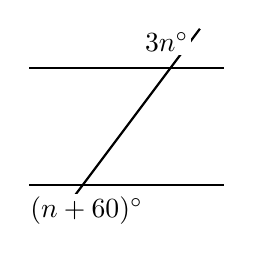
\begin{tikzpicture}[scale=0.62,baseline=(current bounding box.center)]
\draw[thick] (-2,1.2)--(2,1.2);
\draw[thick] (-2,-1.2)--(2,-1.2);
\draw[thick] (-1.5,-2)--(1.5,2);
\node[fill=white,inner sep=1pt] at (0.82,1.72) {$3n^\circ$};
\node[fill=white,inner sep=1pt] at (-0.82,-1.72) {$(n+60)^\circ$};
\end{tikzpicture}}\end{column}
\end{columns}
\vspace{0.45em}
\begin{columns}[T,onlytextwidth]
\begin{column}{0.32\textwidth}\MMProblem{7}{Are the lines parallel? Explain. One pair of corresponding angles is \mbox{$76^\circ$} and \mbox{$76^\circ$}.}\end{column}
\begin{column}{0.32\textwidth}\MMProblem{8}{Are the lines parallel? Explain. One pair of alternate angles is \mbox{$121^\circ$} and \mbox{$59^\circ$}.}\end{column}
\begin{column}{0.32\textwidth}\MMProblem{9}{Are the lines parallel? Explain. A pair of co-interior angles is \mbox{$112^\circ$} and \mbox{$68^\circ$}.}\end{column}
\end{columns}
\end{frame}
\begin{frame}[t]
\WorksheetTitle{Build Tasks}
\vspace{-0.18em}
\begin{columns}[T,onlytextwidth]
\begin{column}{0.32\textwidth}\MMProblem{1}{One acute angle on the diagram is \mbox{$38^\circ$}. List the other three acute/obtuse angle sizes in the diagram.}\end{column}
\begin{column}{0.32\textwidth}\MMProblem{2}{The obtuse angle is \mbox{$143^\circ$}. What is the matching corresponding angle and what is the supplementary acute angle?}\end{column}
\begin{column}{0.32\textwidth}\MMProblem{3}{A student says co-interior angles are equal. Correct the statement in one sentence.}\end{column}
\end{columns}
\vspace{0.45em}
\begin{columns}[T,onlytextwidth]
\begin{column}{0.32\textwidth}\MMProblem{4}{}\end{column}
\begin{column}{0.32\textwidth}\MMProblem{5}{}\end{column}
\begin{column}{0.32\textwidth}\MMProblem{6}{}\end{column}
\end{columns}
\vspace{0.45em}
\begin{columns}[T,onlytextwidth]
\begin{column}{0.32\textwidth}\MMProblem{7}{}\end{column}
\begin{column}{0.32\textwidth}\MMProblem{8}{}\end{column}
\begin{column}{0.32\textwidth}\MMProblem{9}{}\end{column}
\end{columns}
\end{frame}
\end{document}
